\begin{atiTask}[
	title = Eine Zombieapokalypse,
	language = Deutsch
]
	Auf einer kleinen Insel gerät ein Virus in Umlauf, der die Bevölkerung in Zombies verwandelt.
	Jeder Infizierte hat in einer Zeitspanne $\tau\in\setR^+$ Kontakt mit $\tau\cdot k$ anderen Personen, die teilweise ebenfalls infiziert, teilweise aber auch gesunde Menschen sind, wobei $k\in\setR^+$ gilt.
	Gerät ein gesunder Mensch in Kontakt mit einem Zombie, so wird dieser infiziert.
	\medskip
	\begin{atiSubtasks}
		\item{\locallabel{a}
			Stellen Sie eine Differentialgleichung auf, die dieser Zombieapokalypse genügt.
			Verwenden Sie $N\in\setN$ für die Größe der Inselbevölkerung, $Z(t)\in[0,N]$ für die Anzahl der Infizierten, $M(t)\in[0,N]$ für die Anzahl der Gesunden und $t\in\setR^+$ als freien Parameter der Zeit.

			\begin{atiNote}
				Betrachten Sie zunächst nur die Infizierten zum Zeitpunkt $t+\tau$ und überführen Sie die Differenzengleichung durch Grenzwertbildung in die gesuchte Differentialgleichung.
			\end{atiNote}
		}
		\item{\locallabel{b}
			Lösen Sie diese Differentialgleichung und das folgende Anfangswertproblem.
			\[
				t_0\define 0\separate Z_0\define Z(0) \define \frac{N}{21}
			\]
		}
		\item{\locallabel{c}
			Skizzieren Sie $Z(t)$ und $M(t)$ für $k=2$, $N=1050$ und $t\in\setR^+$.
		}
		\item{\locallabel{d}
			\textbf{Zusatz:} Ab wann ist nur noch weniger als $1\unit{\%}$ der Bevölkerung nicht infiziert?
			Wie beeinflussen die Parameter $k$ und $N$ diesen Zeitpunkt?
		}
	\end{atiSubtasks}
\end{atiTask}
\begin{atiSolution}
	\begin{atiSubtaskSolutions}
		\item[\localref{a}]{
			Wir definieren als Erstes den Anteil der gesunden Menschen $\alpha(t)\in[0,1]$ und den Anteil der infizierten Menschen $\beta(t)\in[0,1]$ für alle $t\in\setR^+$.
			\[
				\alpha(t)\define \frac{M(t)}{N}\separate\beta(t)\define\frac{Z(t)}{N}
			\]
			Wir wählen nun eine festen Zeitpunkt $t\in\setR^+$.
			Nähern wir für kleine Zeitspannen $\tau\in\setR^+$ die Anzahl der Personen, die ein Zombie trifft, durch $\tau k$ an, so teilen sich Infizierte und Gesunde entsprechend ihrer Anteile auf diese Anzahl auf.
			% Trifft eine infizierte Person für kleine $\tau\in\setR^+$ nun $\tau k$ andere Personen, so teilen sich Infizierte und Gesunde entsprechend ihrer Anteile $\alpha(t)$ und $\beta(t)$ auf diese Anzahl auf.
			\[
				\tau k \approx \tau k\alpha(t) + \tau k\beta(t)
			\]
			Die Anzahl $S(t)$ der gesunden Menschen, die ein Zombie in der Zeitspanne $\tau$ trifft und infiziert, kann demnach wie folgt für kleine $\tau$ approximiert werden.
			\[
				S(t) \approx \tau k \alpha(t) = \frac{\tau k}{N} M(t)
			\]
			Diese Approximation gilt für jeden Zombie.
			Dementsprechend lässt sich nun die Anzahl der Zombies $Z(t+\tau)$ nach der Zeitspanne $\tau$ beschreiben.
			% Damit ergibt sich die Gesamtanzahl $\Delta Z(t)$ der gesunden Menschen, die während dieser Zeitspanne $\tau$ infiziert werden, durch eine Multiplikation von $S(t)$ mit der Anzahl aller Zombies $Z(t)$.
			% \[
			% 	\Delta Z(t) = S(t)Z(t) = \tau k\alpha(t)Z(t) = \frac{\tau k}{N}M(t)Z(t) = \frac{\tau k}{N} \boxb{N-Z(t)}Z(t)
			% \]
			\[
				Z(t+\tau) \approx Z(t) + S(t)Z(t) = Z(t) + \frac{\tau k}{N} \boxb{N-Z(t)}Z(t)\atiPoints[1]
			\]
			\[
				\implies \frac{Z(t+\tau)-Z(t)}{\tau} \approx \frac{k}{N}\boxb{N-Z(t)}Z(t)
			\]
			Um die Fehler der Näherung mithilfe einer Differentialgleichung zu korrigieren, bildet man den Grenzwert der erhaltenen Differenzengleichung für $\tau\conv 0$.
			\[
				Z'(t) = \lim_{\tau\conv 0}\frac{Z(t+\tau)-Z(t)}{\tau} = \frac{k}{N}\boxb{N-Z(t)}Z(t)
			\]
			\[
				\implies Z' = \frac{k}{N}(N-Z)Z \atiPoints[1]
			\]
		}
		\item[\localref{b}]{
			Bei der oben beschriebenen Gleichung handelt es sich offensichtlich um eine separable Differentialgleichung.
			Die Methode der Trennung der Variablen ergibt dann das Folgende.
			\[
				\frac{Z'(t)}{\boxb{N-Z(t)}Z(t)} = \frac{k}{N} \implies \integral{t_0}{t}{\frac{Z'(s)}{\boxb{N-Z(s)}Z(s)}}{s} = \integral{t_0}{t}{\frac{k}{N}}{s}
			\]
			\[
				\implies \integral{Z_0}{Z(t)}{\frac{1}{(N-s)s}}{s} = \frac{k}{N}(t-t_0)\atiPoints[1]
			\]
			Für die Lösung des Integrals zeigt sich eine Partialbruchzerlegung als sinnvoll.
			\[
				\frac{1}{(N-s)s} = \frac{N}{N}\frac{1}{(N-s)s} = \frac{1}{N}\frac{N-s+s}{(N-s)s} = \frac{1}{Ns} - \frac{1}{N(s-N)}
			\]
			\[
				\implies \integral{Z_0}{Z(t)}{\frac{1}{(N-s)s}}{s} = \integral{Z_0}{Z(t)}{\frac{1}{Ns}}{s} - \integral{Z_0}{Z(t)}{\frac{1}{N(s-N)}}{s}
			\]
			\[
				= \frac{1}{N}\ln\boxb{\frac{Z(t)}{Z_0}} - \frac{1}{N}\ln\boxb{\frac{Z(t)-N}{Z_0-N}} = \frac{1}{N}\ln\curvb{\frac{Z(t)\boxb{Z_0-N}}{Z_0\boxb{Z(t)-N}}}\atiPoints[+1]
			\]
			Die Lösung des Integrals wird nun eingesetzt und die entstehende Gleichung wird explizit nach $Z(t)$ umgestellt.
			\[
				\frac{Z(t)}{Z(t)-N} = \frac{Z_0e^{k(t-t_0)}}{Z_0-N} = -Ae^{k(t-t_0)}\separate A\define \frac{Z_0}{N-Z_0}
			\]
			\[
				\implies Z(t) = \frac{NAe^{k(t-t_0)}}{1 + Ae^{k(t-t_0)}} = N\curvb{1 - \frac{1}{1+Ae^{k(t-t_0)}}}\atiPoints[1]
			\]
			Nun setzen wir die Anfangswerte ein und unterstreichen unser Ergebnis doppelt.
			\[
				A = \frac{1}{20} \implies Z(t) = N\curvb{1 - \frac{1}{1+\frac{1}{20}e^{kt}}}\atiPoints[1]
			\]
		}
		\item[\localref{c}]{
			Die nachfolgende Skizze zeigt die Werte $M(t)$ und $Z(t)$ für verschiedene Zeiten $t\in\setR^+$.
		}
		\item[\localref{d}]{
			Es sei $\alpha^*\in\curvb{0,1-\frac{Z_0}{N}}$ eine feste Grenze für den Anteil der Menschen.
			Wir suchen nun den frühesten Zeitpunkt $t^*\in\setR^+$, sodass $\alpha(t^*)\leq\alpha^*$ gilt.
			Durch Äquivalenzumformungen zeigt man, dass $t^*$ existiert und eindeutig ist.
			\[
				\alpha^* = \alpha(t^*) = 1-\beta(t^*) = 1 - \frac{Z(t^*)}{N} = \frac{1}{1 + Ae^{k(t^*-t_0)}}
			\]
			\[
				\implies t^* = t_0 + \frac{1}{k}\ln\boxb{\frac{1}{A}\curvb{\frac{1}{\alpha^*}-1}} = t_0 + \frac{1}{k}\ln\boxb{\frac{N-Z_0}{Z_0}\curvb{\frac{1}{\alpha^*}-1}}
			\]
			Setzt man nun die gewünschten Werte der Parameter ein, so erhält man das folgende Ergebnis.
			\[
				t_0 = 0\separate k=2\separate A = 0.05 \separate\alpha^* = 1\unit{\%}\implies t^* = \frac{\ln 1980}{2} \approx 3.8\atiPoints[+1]
			\]
			Zu beachten ist, dass $t^*$ sowohl von $k$ als auch von $N$ abhängig ist.
			Steigt $k$, so verringert sich $t^*$.
			Steigt $N$, so erhöht sich auch $t^*$.\atiPoints[+1]
		}
	\end{atiSubtaskSolutions}
	\begin{figure}[H]
		\center
		\atiPoints[2]
		% GNUPLOT: LaTeX picture with Postscript
\begingroup
  \makeatletter
  \providecommand\color[2][]{%
    \GenericError{(gnuplot) \space\space\space\@spaces}{%
      Package color not loaded in conjunction with
      terminal option `colourtext'%
    }{See the gnuplot documentation for explanation.%
    }{Either use 'blacktext' in gnuplot or load the package
      color.sty in LaTeX.}%
    \renewcommand\color[2][]{}%
  }%
  \providecommand\includegraphics[2][]{%
    \GenericError{(gnuplot) \space\space\space\@spaces}{%
      Package graphicx or graphics not loaded%
    }{See the gnuplot documentation for explanation.%
    }{The gnuplot epslatex terminal needs graphicx.sty or graphics.sty.}%
    \renewcommand\includegraphics[2][]{}%
  }%
  \providecommand\rotatebox[2]{#2}%
  \@ifundefined{ifGPcolor}{%
    \newif\ifGPcolor
    \GPcolorfalse
  }{}%
  \@ifundefined{ifGPblacktext}{%
    \newif\ifGPblacktext
    \GPblacktexttrue
  }{}%
  % define a \g@addto@macro without @ in the name:
  \let\gplgaddtomacro\g@addto@macro
  % define empty templates for all commands taking text:
  \gdef\gplbacktext{}%
  \gdef\gplfronttext{}%
  \makeatother
  \ifGPblacktext
    % no textcolor at all
    \def\colorrgb#1{}%
    \def\colorgray#1{}%
  \else
    % gray or color?
    \ifGPcolor
      \def\colorrgb#1{\color[rgb]{#1}}%
      \def\colorgray#1{\color[gray]{#1}}%
      \expandafter\def\csname LTw\endcsname{\color{white}}%
      \expandafter\def\csname LTb\endcsname{\color{black}}%
      \expandafter\def\csname LTa\endcsname{\color{black}}%
      \expandafter\def\csname LT0\endcsname{\color[rgb]{1,0,0}}%
      \expandafter\def\csname LT1\endcsname{\color[rgb]{0,1,0}}%
      \expandafter\def\csname LT2\endcsname{\color[rgb]{0,0,1}}%
      \expandafter\def\csname LT3\endcsname{\color[rgb]{1,0,1}}%
      \expandafter\def\csname LT4\endcsname{\color[rgb]{0,1,1}}%
      \expandafter\def\csname LT5\endcsname{\color[rgb]{1,1,0}}%
      \expandafter\def\csname LT6\endcsname{\color[rgb]{0,0,0}}%
      \expandafter\def\csname LT7\endcsname{\color[rgb]{1,0.3,0}}%
      \expandafter\def\csname LT8\endcsname{\color[rgb]{0.5,0.5,0.5}}%
    \else
      % gray
      \def\colorrgb#1{\color{black}}%
      \def\colorgray#1{\color[gray]{#1}}%
      \expandafter\def\csname LTw\endcsname{\color{white}}%
      \expandafter\def\csname LTb\endcsname{\color{black}}%
      \expandafter\def\csname LTa\endcsname{\color{black}}%
      \expandafter\def\csname LT0\endcsname{\color{black}}%
      \expandafter\def\csname LT1\endcsname{\color{black}}%
      \expandafter\def\csname LT2\endcsname{\color{black}}%
      \expandafter\def\csname LT3\endcsname{\color{black}}%
      \expandafter\def\csname LT4\endcsname{\color{black}}%
      \expandafter\def\csname LT5\endcsname{\color{black}}%
      \expandafter\def\csname LT6\endcsname{\color{black}}%
      \expandafter\def\csname LT7\endcsname{\color{black}}%
      \expandafter\def\csname LT8\endcsname{\color{black}}%
    \fi
  \fi
    \setlength{\unitlength}{0.0500bp}%
    \ifx\gptboxheight\undefined%
      \newlength{\gptboxheight}%
      \newlength{\gptboxwidth}%
      \newsavebox{\gptboxtext}%
    \fi%
    \setlength{\fboxrule}{0.5pt}%
    \setlength{\fboxsep}{1pt}%
\begin{picture}(6802.00,3968.00)%
    \gplgaddtomacro\gplbacktext{%
      \csname LTb\endcsname%
      \put(726,704){\makebox(0,0)[r]{\strut{}$0$}}%
      \put(726,1270){\makebox(0,0)[r]{\strut{}$200$}}%
      \put(726,1836){\makebox(0,0)[r]{\strut{}$400$}}%
      \put(726,2402){\makebox(0,0)[r]{\strut{}$600$}}%
      \put(726,2967){\makebox(0,0)[r]{\strut{}$800$}}%
      \put(726,3533){\makebox(0,0)[r]{\strut{}$1000$}}%
      \put(858,484){\makebox(0,0){\strut{}$0$}}%
      \put(1967,484){\makebox(0,0){\strut{}$1$}}%
      \put(3077,484){\makebox(0,0){\strut{}$2$}}%
      \put(4186,484){\makebox(0,0){\strut{}$3$}}%
      \put(5296,484){\makebox(0,0){\strut{}$4$}}%
      \put(6405,484){\makebox(0,0){\strut{}$5$}}%
    }%
    \gplgaddtomacro\gplfronttext{%
      \csname LTb\endcsname%
      \put(3631,154){\makebox(0,0){\strut{}$t$}}%
      \csname LTb\endcsname%
      \put(5418,2313){\makebox(0,0)[r]{\strut{}$Z(t)$}}%
      \csname LTb\endcsname%
      \put(5418,2093){\makebox(0,0)[r]{\strut{}$M(t)$}}%
    }%
    \gplbacktext
    \put(0,0){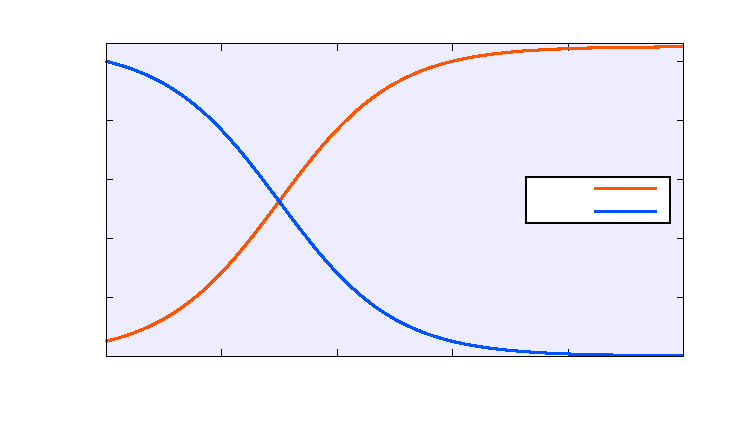
\includegraphics{task-eine_zombieapokalypse-skizze}}%
    \gplfronttext
  \end{picture}%
\endgroup

		\caption*{Die Abbildung zeigt die Anzahl der Zombies $Z(t)$ und der gesunden Menschen $M(t)$ für verschiedene Zeiten $t$.}
	\end{figure}
\end{atiSolution}